\chapter{Introduction}

This tutorial explains in detail how to use the Lightweight IP (from
now on, LWIP) TCP/IP software stack \cite{LWIP} together with \rtd\
and \ee\ for the Altera Nios II platform.

The tutorial is based on the Nios II Standalone LWIP Port available
for download in the Nios Community Forum, and it covers LWIP version
0.7.1. Support for newer versions of LWIP will be added in the next
revision of this document.

At the end of the tutorial, the developer will be able to run a
modified version of the LWIP web server demo on top of an Altera
evaluation board.

The demo fully supports the LWIP RAW API. The rationale behind the
choice is that the RAW API is an event based interface to the TCP/IP
stack that perfectly integrates with the non-blocking task model
provided by \ee. In particular, the LWIP timers and service routines
are mapped to a set of tasks; LWIP and Application tasks can share a
common stack reducing the overall RAM usage.

The socket interface is currently not supported because of bigger
memory requirements, and because of the need of blocking primitives
(e.g., \fn{select}) that would not take advantage of the stack sharing
mechanisms of \ee.

If compared to the single task LWIP standalone version for the Altera
HAL\footnote{The LWIP standalone version for the Altera HAL is
available for free in the Nios II Community Forum Download area.},
this porting of the LWIP stack fully supports the multithread
environment of \ee, meaning that application task can run
together with LWIP tasks.

For more information about the LWIP example and on the LWIP internals,
please refer to the original \file{readme.txt} included in the
distribution.

The structure of this tutorial is the following: Chapter
\ref{cha:Requirements} contains the requirements for installing the
LWIP port for \ee; Chapter \ref{cha:Running-the-demo} is
a step-by-step guide for the installation, configuration and run of
the demo; finally, Chapter \ref{cha:Advanced-configuration} contains
advanced configuration issues.


\chapter{Requirements}
\label{cha:Requirements}

The LWIP demo presented in this tutorial requires the following
software to be installed on the host machine:

\begin{itemize}
\item Altera Quartus II version 5.0;
\item Altera Nios II version 5.0;
\item \rtd\ and \ee\ for Nios II version 1.2.5. The evaluation version
  of the tools will {\em not} work straightforward because they
  require a 2-CPU demo, whereas this tutorial is based on the
  \const{standard} Altera examples.
\item Standalone Lightweight IP version 1.1 (available on the Nios II
  Community Forum).
\item This example requires an Ethernet cable connected to the
  development board's RJ-45 jack, and a JTAG connection with the
  development board. If the host communication settings are changed
  from JTAG UART (default) to use a conventional UART, a serial cable
  between board DB-9 connector and the host is required.

\end{itemize}

The demo will work on the standard and full featured demos available
for the Altera Evaluation boards.


\chapter{Running the LWIP Demo\label{cha:Running-the-demo}}

The following basic steps will guide you in running a small web server
using the LWIP TCP/IP stack:

\begin{enumerate}
\item Open the \file{standard} example for your evaluation board from
  Altera Quartus II.
\item Open SOPCBuilder, by double clicking on the SOPCBuilder
  Block. Then, open the Nios II IDE.
\item Create a new Altera System Library Project. Call it
  \const{standard\_syslib}. See Figure \ref{fig:lwip_system_library}
  for a screenshot.
%
\begin{figure}
\begin{center}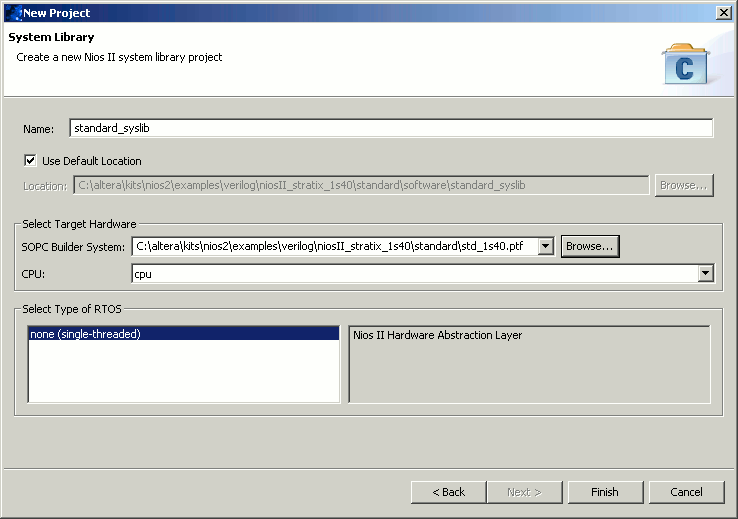
\includegraphics[%
  width=10cm, bb=0 0 738 519]{images/lwip_system_library.png}\end{center}

\caption{\label{fig:lwip_system_library}This screenshot shows the
dialog box for the creation of the \const{standard\_syslib} project.}
\end{figure}
%
\item Then, select ``New Project...''  from the File menu. Choose
  ``\rtd\ Nios Project'' from the Evidence tab of the New Project
  Dialog box. A dialog box appears.  Name the project \file{evidence_lwip}
  and press the Finish button.
%
\begin{figure}
\begin{center}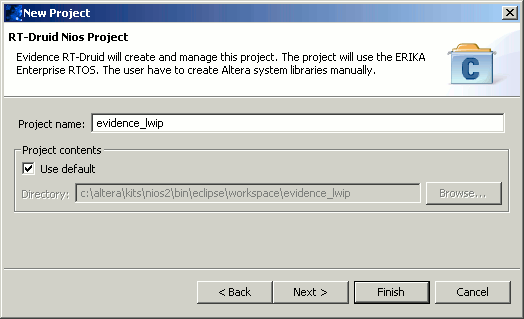
\includegraphics[%
  width=10cm, bb=0 0 524 319]{images/lwip_rtdruid_project.png}\end{center}

\caption{\label{fig:lwip_rtdruid_project}This screenshot shows the
dialog box for the creation of the \rtd\ Project.}
\end{figure}
%
\item Select ``Import...'' from the File menu of the Nios II
  IDE. Select ``File System'' from the dialog box. In the ``From
  directory'' textbox, type the name of the \file{src} directory
  included the example you downloaded from the Evidence website (you
  can also select it using the ``Browse'' button). Choose the
  directory name in the tree view on the left, selecting all the files
  on the right side. The ``Into Folder'' text box should point to the
  \file{evidence_lwip} demo. Finally, select the checkbox ``Overwrite
  existing resources without warning'' and press Finish. See Figure
  \ref{fig:lwip-import-filesystem} for a screenshot of the Import
  window.
%
\begin{figure}
\begin{center}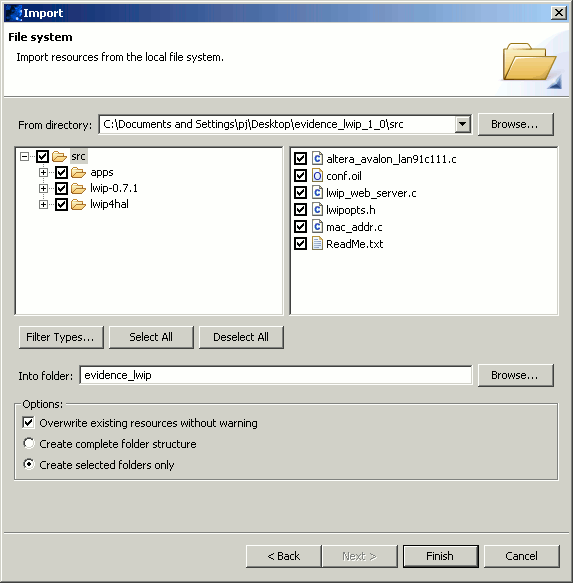
\includegraphics[%
  width=10cm, bb=0 0 573 583]{images/lwip_import_filesystem.png}\end{center}

\caption{\label{fig:lwip_import_filesystem}This screenshot shows the
dialog box for the import of the demo inside the current project.}
\end{figure}
%
\item Among the files that have been imported in the \rtd\ Project,
  find the file named \file{altera\_avalon\_lan91c111.c}. You have to
  copy it into the System Library Project \file{standard\_syslib}. To
  copy it, right click on the file name, and choose ``Copy''; then,
  right click on the project name, and select ``Paste''. The file you
  just copied will replace the file provided by default by the
  Standalone LWIP package. The new file is equal to the previous one
  apart for a callback that has been added to the IRQ handler
  function.
\item Right click on the System Library name, and choose ``Build
  Project'' to build the System Library.
\item Set up the \rtd\ project build directory. To do that,
  open the properties of the project, and inside the ``C/C++ Make
  Project'' tab, in the Build directory textbox, specify
  \file{\\<projectname>\\Debug}, where \file{<projectname>} is the
  name of the project. See Figure \ref{fig:lwip-properties-make} for
  details.
%
\begin{figure}
\begin{center}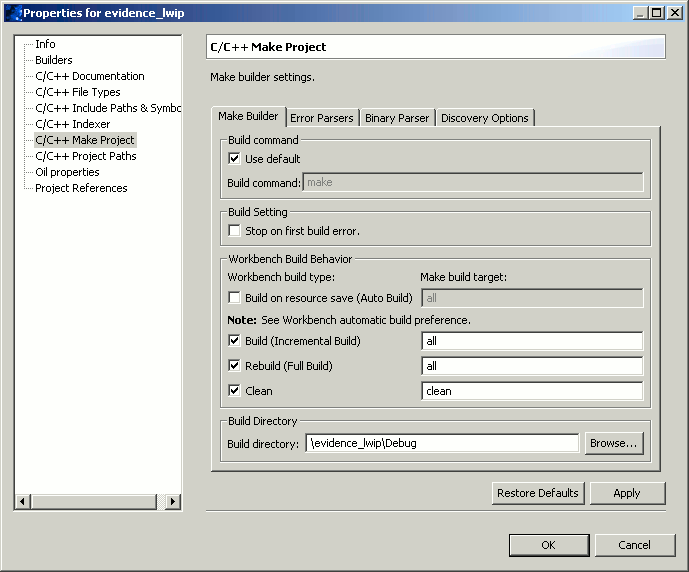
\includegraphics[%
  width=8cm, bb=0 0 689 572]{images/lwip_properties_make.png}\end{center}
\caption{\label{fig:lwip-properties-make}Changing the Project Build
Directory. You can insert the value pressing the Browse button.}
\end{figure}
%
\item Find and edit the IP address, network mask, and gateway address
  inside the file \file{lwip_web_server.c}. You will use this address
  from your web browser to test the application.

\item After that, right click on the \rtd\ project name, and select
  ``Build Project''.  The demo application will be compiled, and an
  ELF binary file will be produced.
%
\item Open the Altera Quartus II Programmer from the ``Tools''
  menu. Select the right \file{standard.sof} file, and program it to
  the FPGA. The hardware design is now programmed to the FPGA.

\item In the ``Run'' menu, click on the ``Run...'' command. 

\item Create a Run configuration as shown in Figure
  \ref{fig:lwip-run-configuration}.
%
\begin{figure}
\begin{center}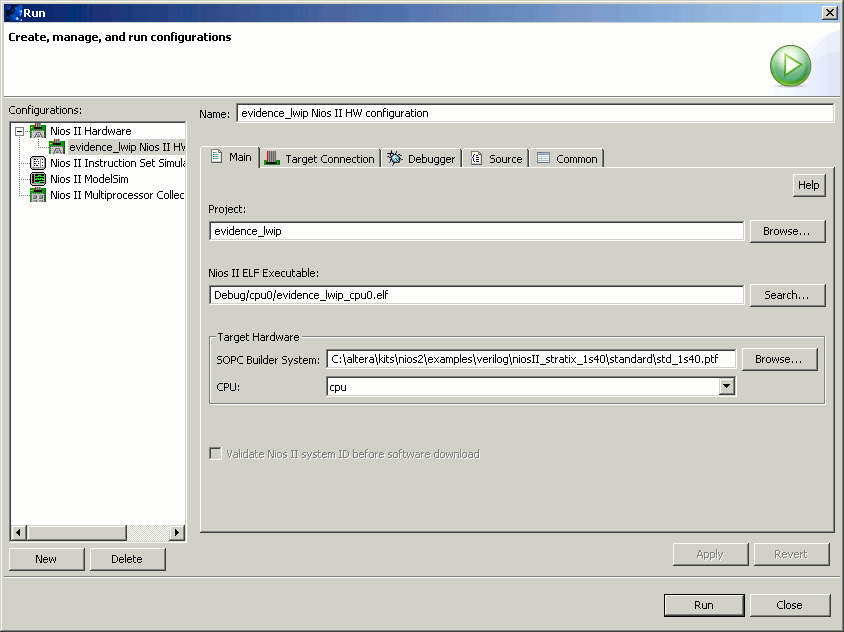
\includegraphics[%
  width=8cm, bb=0 0 844 632]{images/lwip_run_configuration.png}\end{center}
\caption{\label{fig:lwip-run-configuration}You need to create a
Debug/Run configuration to be able to run the application on the
target.}
\end{figure}
%
\item Run the application by clicking on the ``Run'' button in Figure
  \ref{fig:lwip-run-configuration}. As a result, the application
  starts printing some text on the console like in Figure
  \ref{fig:lwip-console}.
%
\begin{figure}
\begin{center}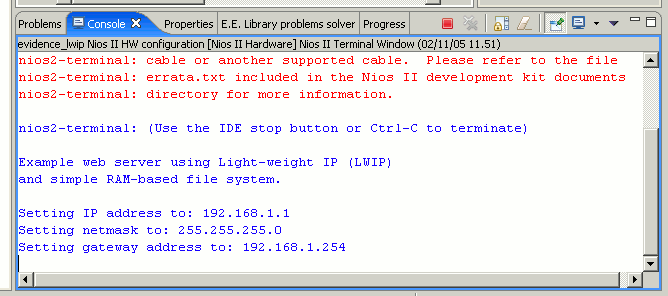
\includegraphics[%
  width=8cm, bb=0 0 844 632]{images/lwip_console.png}\end{center}
\caption{\label{fig:lwip-console}The messages printed on the JTAG UART
console.}
\end{figure}
%
\item Obtaining the messages in Figure \ref{fig:lwip-console} means
  the web server is up and running.At that point, you can do the
  following actions:
  \begin{itemize}
    \item Browse the server using this IP address in the address bar
      of your browser.
    \item Use a Telnet client to connect to TCP port 7 to exercise the
      echo function.
    \item Use Ping with a length greater than 1500 and less than 5500
      bytes to exercise the IP reassembly and fragmentation
      capability.
  \end{itemize}
\end{enumerate}



\chapter{Configuration of the RTOS parameters for the LWIP stack}
\label{cha:Advanced-configuration}

\section{Application structure}

When using the LWIP TCP/IP stack together with \ee, the
application design have to be designed accordingly to a set of common
sense rules that help handling the TCP/IP with the least overhead
maintaining the possibility of having concurrent tasks running in the
system. These rules are shortly described below (see Figure
\ref{fig:lwip:interrupts} for a graphical reference), and are used in
the demo distributed together with this tutorial.

%
\begin{figure}
\includegraphics[%
  width=1\columnwidth]{images/lwip_interrupts.eps}
\caption{\label{fig:lwip-interrupts}This Figure displays the
architecture of the LWIP port, showing the timer and LAN interrupts,
the LWIP tasks, and the main task.}
\end{figure}

\begin{itemize}
\item The \fn{main()} function is used for \ee\ initialization
  purposes {\em only}. In general, that function covers the system
  startup and implements at its end the background processing. For
  that reason, it should not call any LWIP timer function after system
  initialization (please note that the standalone example distributed
  in the Nios II Community forum does all the processing inside the
  \fn{main()}). The rationale for this choice is that the application
  designer should be able to specify the precedence the application
  tasks should have over the TCP/IP processing.
\item The initialization phase is carried out by a task named
  \fn{LWIP_startup_task}, that basically contains all the
  initialization routines of the LWIP stack. The task is automatically
  activated by the \fn{StartOS()} primitive (the \const{AUTOSTART}
  property of the task is set to \const{TRUE} in the OIL file.
\item There are other two tasks, named \fn{LWIP_service_task} and
  \fn{LWIP_timer_task}, that are responsible to the execution of the
  LWIP timer functions. The rationale behind this choice is that the
  RAW API exports an event-based API for the handling of TCP/IP. There
  are two kind of events in the LWIP code: periodic and asynchronous
  events, with corresponding periodic and asynchronous LWIP timer
  functions. Periodic events are handled every given amount of time to
  process TCP, ARP, and reassembly timeouts. Asynchronous events occur
  in correspondence of the process of incoming packets from the
  network interface.
\item The \fn{LWIP_service_task} task simply calls the
  \fn{lan91c111if_service} that is used by the LWIP stack to process
  an incoming packet. In principle, the \fn{LWIP_service_task} task is
  activated every interrupt from the Ethernet interface\footnote{That
  is the reason for the patch to \fn{alt_avalon_lan91c111_irq()}.The
  actual implementation slightly differ because there is to consider a
  race condition between task activation and the service process of
  the packet.}. Please note that the standalone version called
  \fn{lan91c111if_service} in the main loop, which typically resulted
  in a lot of computation time spent inside the call without any
  packet arrived, or, worse, since real application in the standalone
  version have to be implemented inside the main loop, having a lot of
  computation inside \fn{main} simply decrease the polling frequency
  of the network, with a result of delays in the packet handling.
\item The \fn{LWIP_timer_task} task is activated periodically using an HAL
  alarm. The alarm mechanism of the Altera HAL is usually attached to
  the system timer. The content of he task is basically a call to all
  the periodic timeouts that handle the TCP/IP stack.
\item The priorities of the three LWIP tasks are all the same, to
  avoid preemption between different LWIP tasks.
\item Processing into the ISRs is reduced to the minimum possible, to
  avoid long interval of time executed with interrupt disabled: de
  facto, they contain only a call to \fn{ActivateTask()}. Once
  activated, the LWIP tasks are scheduled like other application
  tasks, eventually sharing the stack with them to reduce the overall
  RAM consumption while maintaining multithread capabilities.
\end{itemize}

As a result, the application architecture depicted in the previous
points allow multitasking support without loosing the efficiency of
the RAW API, and enabling stack sharing between application tasks and
LWIP tasks.

\section{Handling concurrency between LWIP calls}

Application tasks typically need to use the LWIP API only to create,
bind, and listen on connections. All the other processing will be done
on packet arrivals and on the periodic timers, that are handled inside
the \fn{LWIP_service_task} and \fn{LWIP_timer_task} LWIP tasks. 

The developer have also to take care of a race condition that appears
when passing from the standalone version of the LWIP stack to a
multitask system. In particular, some care have to be taken to avoid
that the LWIP tasks \fn{LWIP_service_task} and \fn{LWIP_timer_task}
preempts the running task during a LWIP call.

To avoid that situation, one out of the following four strategies can
be implemented:

\begin{enumerate}
\item The LWIP tasks can be assigned the highest priority in the
  system. Then, a Resource is allocated, that is shared among the LWIP
  tasks and all the application tasks that needs to call the LWIP
  API. All the calls to the LWIP API done by application tasks have to
  be protected by the usage of the resource.

  As a result, the two LWIP tasks have the same priority, and so they
  are in mutual exclusion {\em without} the need of calling
  \fn{GetResource()} and \fn{ReleaseResource()}. Then, when a task
  uses a LWIP API function, the call of \fn{GetResource()} before the
  usage of the API functions has the result of increasing the running
  task priority to the ceiling of the resource\footnote{\ee\ uses the
  Immediate Priority Ceiling Protocol, which says that the ceiling of
  a resource is the highest priority of the tasks potentially using
  the resource. Resource usages are taken from the OIL file.}, making
  the task mutually exclusive with the LWIP tasks. If a packet arrives
  or a LWIP timeout expires while the running task executes the API
  function, then the LWIP task will be activated, and will then wait
  the release of the resource done by the running task with a call to
  \fn{ReleaseResource()}.

  Please note that the demo distributed with this tutorial implements
  this scheme.

\item The LWIP tasks have not the highest priority in the system. In
  this case {\em all} the calls to the LWIP API, and the code of the
  LWIP tasks have to be protected using a shared resource.

\item All the task using the LWIP API can be defined in the OIL file
  as non preemptive. In this case, no explicit call to
  \fn{GetResource()} and \fn{ReleaseResource()} is needed. Note
  that other tasks with a priority higher than the LWIP tasks may
  suffer a blocking time also if they do not use the LWIP stack.

\item All the tasks using the LWIP API can be defined in the OIL file
  to share an internal resource. Also in this case, no explicit call
  to \fn{GetResource()} and \fn{ReleaseResource()} is
  needed. Other higher priority tasks can preempt the LWIP and the
  application tasks using the LWIP API.
\end{enumerate}
% da migliorare con disegni e pezzi di codice
